% file: ot-tcs06.tex

\documentclass[tikz]{standalone}

\usetikzlibrary{shapes, positioning, arrows.meta, calc, backgrounds, fit}

\newcommand{\ins}[2]{\textsc{Ins}(#1,#2)}
\newcommand{\del}[2]{\textsc{Del}(#2)}  % del(a, p): ignoring the deleted element ``a''

\begin{document}
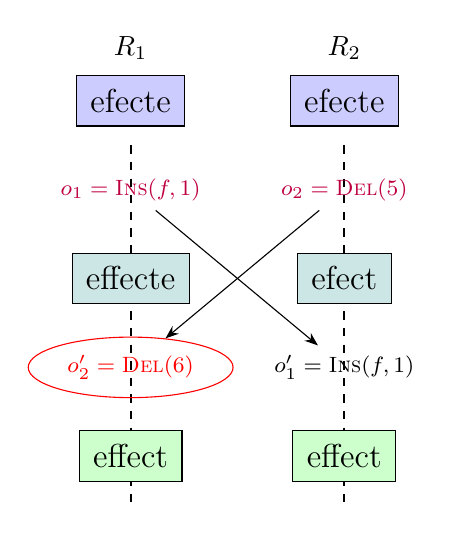
\begin{tikzpicture}[
	timeline/.style = {thick, dashed}, 
	>=Stealth, 
	send/.style = {>=Stealth, ->},
	list/.style = {rectangle, draw, inner sep = 5pt, outer sep = 2pt, fill = #1, font = \large},
	op/.style = {font = \footnotesize, #1}
  ]

  \node[list = blue!20, label = {above:{$R_1$}}] (r1) {efecte}; 
  \node[list = blue!20, right = 1.20cm of r1, label = {above:{$R_2$}}] (r2) {efecte};

  \foreach \r/\rbot in {r1/r1bot, r2/r2bot} {
    \node[below = 4.0cm of \r] (\rbot) {};
  }

  \draw[timeline] ($(r1.south)+(0,-5pt)$) -- ($(r1bot.south)+(0,-15pt)$);
  \draw[timeline] ($(r2.south)+(0,-5pt)$) -- ($(r2bot.south)+(0,-15pt)$);

  \node (ins) [op = purple] at ($(r1)!0.25!(r1bot)$) {$o_1 = \ins{f}{1}$};
  \node (del) [op = purple] at ($(r2)!0.25!(r2bot)$) {$o_2 = \del{e}{5}$};

  \node (r11) [list = teal!20] at ($(r1)!0.50!(r1bot)$) {effecte};
  \node (r21) [list = teal!20] at ($(r2)!0.50!(r2bot)$) {efect};

  \node (ins') [op] at ($(r2)!0.75!(r2bot)$) {$o_1' = \ins{f}{1}$};
  \node (del') [op, red, ellipse, draw] at ($(r1)!0.75!(r1bot)$) {$o_2' = \del{e}{6}$};

  \draw[send] (ins) -- (ins');
  \draw[send] (del) -- (del');

  \node (r12) [list = green!20] at ($(r1)!1.00!(r1bot)$) {effect};
  \node (r22) [list = green!20] at ($(r2)!1.00!(r2bot)$) {effect};
\end{tikzpicture}
\end{document}